\documentclass{VUMIFPSkursinis}
\usepackage{algorithmicx}
\usepackage{algorithm}
\usepackage{algpseudocode}
\usepackage{amsfonts}
\usepackage{amsmath}
\usepackage{bm}
\usepackage{caption}
\usepackage{color}
\usepackage{float}
\usepackage{graphicx}
\usepackage{listings}
\usepackage{subfig}
\usepackage{wrapfig}

\usepackage{enumitem}
%PAKEISTA, tarpai tarp sąrašo elementų
\setitemize{noitemsep,topsep=0pt,parsep=0pt,partopsep=0pt}
\setenumerate{noitemsep,topsep=0pt,parsep=0pt,partopsep=0pt}

% Titulinio aprašas
\university{Vilniaus universitetas}
\faculty{Matematikos ir informatikos fakultetas}
\department{Programų sistemų katedra}
\papertype{Projektinis darbas}
\title{Muzikos kaupimo programos MusiX projektas}
\titleineng{}
\status{2 kurso studentai}
\author{Dominykas Paulikas}
 \secondauthor{Matas Kirvaitis, Martynos Bernotas}   % Pridėti antrą autorių
\supervisor{Vytautas Valaitis}
\date{Vilnius – \the\year}

% Nustatymai
%\setmainfont{Palemonas}   % Pakeisti teksto šriftą į Palemonas (turi būti įdiegtas sistemoje)
\bibliography{bibliografija}

\begin{document}
	
% PAKEISTA	
\maketitle
\cleardoublepage\pagenumbering{arabic}
\setcounter{page}{2}

%TURINYS
\tableofcontents

\sectionnonum{Įvadas}
Šio darbo tikslas yra suprojektuoti intuityvią, naudotojui aiškią ir nesunkiai naudojamą, greitai veikiančią muzikos kaupimo programą. Ši programa naudotojo pateiktą nuorodą į muzikinį kūrinį prideda į jo sudarytus grojaraščius ir leidžia jų klausytis ne tik platformoje, kurioje buvo įvykdytas kūrinio pasirinkimas, bet ir kitose platformose ar įrenginiuose. MusiX veiks Windows bei Android operacinėse sistemose, vartotojui prisijungus prie savo paskyros jo dainos bei grojaraščiai bus randami visuose programą palaikainčiuose įrenginiuose. MusiX programa yra išskirtinė tuo, kad padaro tai, ko kitos šiuo metu egzistuojančios muzikos klausymo platformos nesugeba įgyvendinti ar įgyvendina limituotai - kaupti savąją dainų kolekciją iš įvairių šaltinių. Kai kurios platformos už jų siūlomos muzikinės bibliotekos papildymą pačių programos naudotojų turimais kūriniais prašo mėnesinių mokesčių ar yra išvis draudžiamos Lietuvoje bei daugelyje kitų šalių. Šis projektas bando pašalinti šiuos limitus, leisdamas nesunkiai kurti savą muzikos kolekciją be papildomų mokesčių ar draudimų. Šiuo projektu siekiama palengvinti muzikos megėjų, saugančių savo muzikinę kolekciją daugybėje skirtingų vietų, gyvenimus leidžiant jiems apjungti įvairius muzikos ar kitų garso takelių šaltinius. Tikimasi, kad galų gale MusiX bus pagrindinė bei mėgiamiausia ne tik Lietuvių, bet ir kitų šalių gyventojų muzikinė platforma.

\section{Sistemos reikalavimai}

\subsection{Funkciniai reikalavimai}
Čia pateikiami reikalavimai apibrėžia pagrindines ir pagalbines sistemos funkcijas. 

\begin{enumerate}[start=1,label={\bfseries FR\arabic*}]
\item Programa turi atlikti šiuos naudotojo prijungimo veiksmus:
	\begin{enumerate}[start=1,label={\bfseries FR1.\arabic*}]
	\item Programa turi užregistruoti naudotoją.
	\item Programa turi prijungti naudotoją.
	\item Programa turi padėti naudotojui atgauti pamirštą slaptažodį.
	\end{enumerate}
\item Programa turi atvaizduoti šiuos elementus:
	\begin{enumerate}[start=1,label={\bfseries FR2.\arabic*}]
	\item Programa turi atvaizduoti esančius grojaraščius.
	\item Programa turi atvaizduoti grojaraštyje esančius garso takelius.
	\end{enumerate}
	\item Programa turi atvaizduoti tokius pasirinkto duomenis:
	\begin{enumerate}[start=1,label={\bfseries FR2.3.\arabic*}]
	\item Dainos pavadinimą ir atlikėją.
	\end{enumerate}
\item Programa turi groti pasirinktą garso takelį.
\item Programa turi sustabdyti grojantį garso takelį.
\item Programa turi pertraukti grojantį garso takelį.
\item Programa turi praleisti grojamo garso takelio dalį.
\item Programa turi pridėti naują grojaraštį.
\item Programa turi keisti grojaračio pavadinimą.
\item Programa turi pridėti dainas prie grojaraščio.
\item Programa turi leisti keisti tokius dainos duomenis kaip:
	\begin{enumerate}[start=1,label={\bfseries FR10.\arabic*}]
	\item Dainos pavadinimą ir atlikėją.
	\end{enumerate}
\item Programa turi leisti ištrinti grojaraštį.
\item Programa turi leisti ištrinti dainą iš grojaraščio.
\item Programa turi siųsti naudotojo grojaraščių atnaujinimus į duomenų bazę. Tarp siunčiamų duomenų privalo būti grojaraščio pavadinimas bei grojaraštyje esantys garso takeliai
\item Programa turi atnaujinti vartotojo grojarčio takelius pagal duomenų bazės duomenis.
\item Programa turi siųsti vartotojo dainų duomenų naujinimus į duomenų bazę.
\item Programa turi atnaujinti vartotojo dainas pagal duomenų bazės duomenis.
\end{enumerate}


\subsection{Nefunkciniai reikalavima}
Čia bus pateikiami vidinių interfeisų, veikimo, aptarnavimo, priežiūros, apsaugos reikalavimai, keliami šiai programinei įrangai.

\begin{enumerate}[start=1,label={\bfseries NFR\arabic*}]
\item Sistema naujai užregistruoto naudotojo duomenis turi iškart nusiųsti į duomenų bazę, kur jie turi būti išsaugomi.
\item Naudotojui pageidavus, turi būti galimybė prisijungimo lange paprašyti gauti laikiną slaptažodį į registracijos metu nurodytą elektroninį paštą. Tokiu atveju senasis slaptažodis yra anuliuojamas.
\item Vartotojui prisijungiant jo įvesti duomenys yra patikrinami duomenų bazėje. Jei toks vartotojas randamas, jis yra prijungiamas prie sistemos.
\item Prisijungimo metu sistema turi kreiptis į duomenų bazę ir gauti visus duomenis, reikalingus sklandžiam pagrindinio progamos lango veikimui.
\item Programos atnaujinimai neturi būti leidžiami dažniau nei kas vieną savaitę, nebent sistemoje buvo rasta klaida, gadinanti naudotojų patirtį ar kelianti saugumo pavojų.
\item Duomenų bazės serveris turi būti visuomet įjungtas ir leidžiantis naudotojams bet kuriuo paros metu prisijungti prie sistemos ir naudotis visais jos funkcionalumais. 
\item Dainų ar grojanraščių informacijos pakeitimai turi būti iškarto sinchronizuojami su duomenų baze.
\item Nautotojų slaptažodžiai yra saugomi užšifruotu pavidalu ir yra siunčiami tarp įrenginių bei duomenų bazės tik tokiu pavidalu.
\item Naudotojų elektroniniai paštai nėra užšifruojami.
\item Sistema turi atsakyti į bet kokius vartotojo veiksmus, parodyti pranešimą apie tinkamą arba netinkamą elgesį ar funkcionalumo sutrikimą. 
\item Tarp grojamų dainų visuomet yra 3 sekundžių tarpas, kurio metu turi būti pradedama groti kita pasirinkta daina. Grojimo metu daina yra toliau užkraunama fone ir naudotojoas 
nejaučia jokių dainos trikdžių ar sustojimų.
\item Dainos ar grojaraščių pridėjimas, naikinimas bei keitimas vartotojo sąsajoje matomas iškarto, o padarytų pakeitimų sinchronizavimas su duomenų baze atliekamas fone ir 
negali trukti ilgiau 5-ių sekundžių.
\item Bandant išjungti programą jai tebesinchronizuojantis su duomenų baze, turi būti parodomas pranešimas, prašantis vartotojo palaukti, kol bus baigta sinchronizacija ir programos 
išjungimas turi būti atideliojamas iki sinchronizacijos pabaigos, bet ne ilgiau kaip 5-ioms sekundėms. 
\item Sutrikimus iššaukiančių įvykių procentas turėtų neviršyti 3 procentų. 
\item Sistema turi gebėti savaime atkurti savo funkcionalumą, ypač netikėtai baigus programos darbą dėl nenumatytų situacijų. 
\item Laikas, reikalingas sistemos funkcionalumui atkurit, neturetų būti ilgesnis nei 7-ios sekundės.
\item Programos atnaujinimui nepavykus, programa turi būti grąžinima į pradinė, prieš-atnaujiniminę būseną.
\item Grojaraščių pavadinimai turi būti tokie patys, kaip ir duomenų bazėje. 
\item Pridėjus naują dainą ir neradus tos dainos atitikmens duomenų bazėje, šios dainos pavadinimas yra automatiškai nustatomas į šaltinyje randama pavadinimą. 
\item Sistema geba skirti panašius objektus vieną nuo kito, nepasimeta, jei dviejų dainų ar grojaraščių pavadinimai yra panašūs.
\item Sistema negali pradėti groti kelių kūrinių vienu metu.
\item Grojančios dainos progreso laikmatis turi rodyti dabartinės dainos grojimo laiką minutėmis ir sekundėmis. Visą laiką turi būti rodomas minimaliai vienas minučių simbolis 
(jei daina grojama dar mažiau nei 60 sekundžių, rodomas 0) ir du sekundžių simboliai. 
\item Naudotojui įvedus netinkamą url turėtų būti parodomas pranešimas, nurodantis įvesti tinkamą url. 
\item Sistema turi veikti Windows ir Android aplinkoje.
\item Programos diegimas turi būti nemokamas
\item Programos diegimas neturėtų trukti ilgiau nei 5 minutes
\item Sistema turi būti aiški bet kokio išsilavinimo vartotojui.
\item Vartotojų prisijungimo informacija turi būti konfidenciali ir apsaugota.
\item Vartotojai neturėtų būti skirstomi į klases, visi turi turėti lygias galimybes naudotis sistema.
\item Vartotojų duomenys neturi būti skelbiami viešai.
\item Statistinių duomenų apdorojimas gali būti naudojamas norint pagerinti sistemos veiklą, bet statistika neturi būti skelbiama viešai.
\item Vartotojas neturėtų saugoti muzikos, apribotos autorių teisėmis, bet sąžiningas sistemos naudojimas yra paties vartotojo atsakomybė.
\end{enumerate}

\section{Struktūrinis dalykinės srities modelis}

\begin{figure}[H]
    \centering
    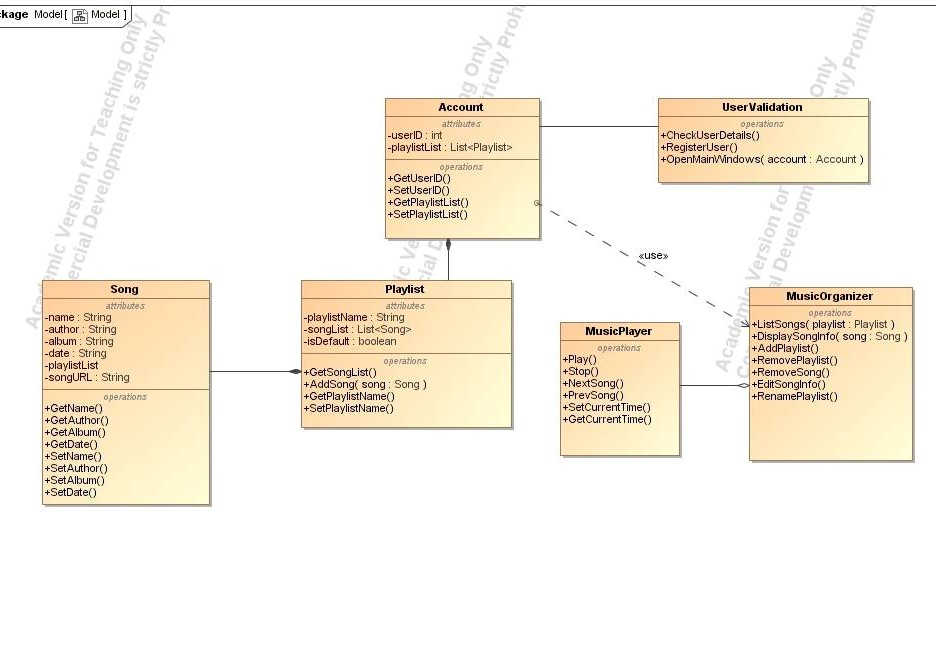
\includegraphics[scale=0.75]{img/Classes}
    \caption{Klasių diagrama}
    \label{img:class}
\end{figure}

Klasių diagramoje, matome programoje veikiančias klases bei jų ryšius. Itin svarbi čia yra MusicOrganizer klasė, kuri valdo didžiają dalį programos veikimo ir yra iššaukiama iškart po sėkmingo prisijungimo. Ji šaukia bei kuria kitus objektus, tokius kaip naujai pridėtos dainos ar grojaraščiai, ir jas nuolatos sinchronizuoja su duomenų baze.

\end{document}
